\documentclass[tikz,border=0pt]{standalone}
%% Shared style for the figures: TUHH colour palette, Latin Modern fonts.
%% Highlights are bold at caption size (10 pt); longer text is regular and
%% 2 pt smaller (8 pt). Figures are drawn at the text width of the
%% manuscript (390 pt) and must be included unscaled.
\usepackage[T1]{fontenc}
\usepackage{lmodern}
\usepackage{graphicx}
\usepackage{tikz}
\usetikzlibrary{arrows.meta,positioning,calc,fit,backgrounds}

\definecolor{tuhhturquoise}{HTML}{00C1D4}
\definecolor{tuhhyellow}{HTML}{FFDE36}
\definecolor{tuhhred}{HTML}{FF4F4F}
\definecolor{tuhhmint}{HTML}{5AFFC5}
\definecolor{tuhhcoolgray}{HTML}{D0D0CE}
\definecolor{tuhhpurple}{HTML}{7200FE}
\definecolor{tuhhwarmgray}{HTML}{A8968C}
\colorlet{ink}{black!85}

\newcommand{\hl}[1]{{\fontsize{10}{12}\selectfont\bfseries #1}}
\newcommand{\tx}[1]{{\fontsize{8}{9.6}\selectfont #1}}
\newcommand{\txi}[1]{{\fontsize{8}{9.6}\selectfont\itshape #1}}

%% \logo{file stem}{height}{fallback wordmark}: uses logos/<stem>.pdf or
%% .png when present, and a typeset wordmark otherwise.
\newcommand{\logo}[3]{%
  \IfFileExists{logos/#1.pdf}{\includegraphics[height=#2]{logos/#1.pdf}}{%
  \IfFileExists{logos/#1.png}{\includegraphics[height=#2]{logos/#1.png}}{%
  {\fontsize{10}{12}\selectfont\bfseries\sffamily #3}}}}

\tikzset{
  x=1pt, y=1pt, text=ink,
  card/.style={draw=tuhhcoolgray, line width=0.8pt, rounded corners=3pt,
               fill=white},
  band/.style={rounded corners=3pt, draw=none},
  flow/.style={-{Stealth[length=5pt,width=4.5pt]}, line width=1pt,
               draw=ink},
  gap/.style={draw=tuhhred, line width=1pt, dash pattern=on 3pt off 2pt},
  lbl/.style={inner sep=0pt, outer sep=0pt, align=left, anchor=north west},
  tag/.style={fill=tuhhyellow, rounded corners=2pt, inner xsep=3pt,
              inner ysep=1.5pt, anchor=west},
}

\begin{document}
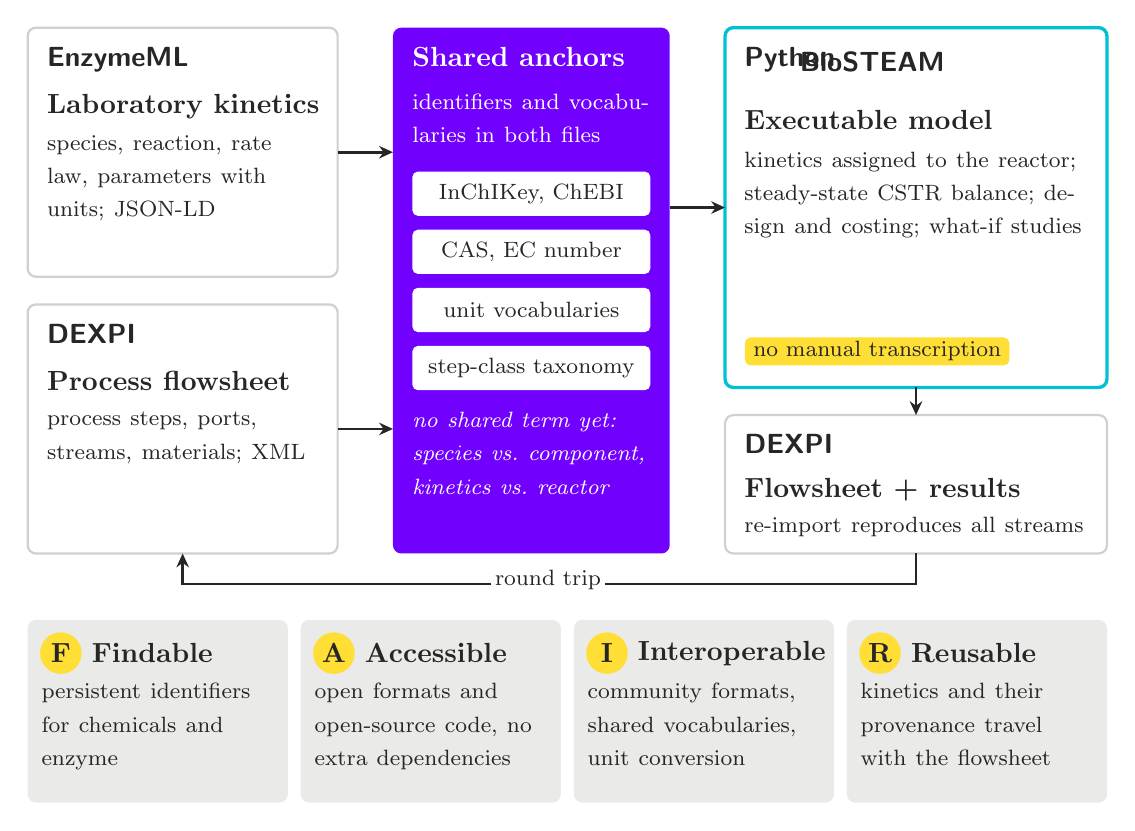
\begin{tikzpicture}
\useasboundingbox (0,0) rectangle (390,280);

% --- inputs ---------------------------------------------------------------
\draw[card] (0,190) rectangle (112,280);
\node[lbl] at (7,273) {\logo{enzymeml}{11pt}{EnzymeML}};
\node[lbl] at (7,256) {\hl{Laboratory kinetics}};
\node[lbl, text width=98pt] at (7,241)
  {\tx{species, reaction, rate law, parameters with units; JSON-LD}};

\draw[card] (0,90) rectangle (112,180);
\node[lbl] at (7,173) {\logo{dexpi}{11pt}{DEXPI}};
\node[lbl] at (7,156) {\hl{Process flowsheet}};
\node[lbl, text width=98pt] at (7,141)
  {\tx{process steps, ports, streams, materials; XML}};

% --- anchors --------------------------------------------------------------
\draw[band, fill=tuhhpurple] (132,90) rectangle (232,280);
\node[lbl, text=white] at (139,273) {\hl{Shared anchors}};
\node[lbl, text=white, text width=86pt] at (139,256)
  {\tx{identifiers and vocabularies in both files}};
\foreach \y/\t in {220/{InChIKey, ChEBI},
                   199/{CAS, EC number}, 178/{unit vocabularies},
                   157/{step-class taxonomy}}{
  \fill[white, rounded corners=2pt] (139,\y-8) rectangle (225,\y+8);
  \node[anchor=center] at (182,\y) {\tx{\t}};
}
\node[lbl, text=white, text width=86pt] at (139,141)
  {\txi{no shared term yet: species vs.\ component, kinetics vs.\ reactor}};

% --- simulator ------------------------------------------------------------
\draw[card, draw=tuhhturquoise, line width=1.2pt] (252,150) rectangle (390,280);
\node[lbl] at (259,273) {\logo{python}{15pt}{Python}};
\node[lbl] at (279,271) {\logo{biosteam}{12pt}{BioSTEAM}};
\node[lbl] at (259,250) {\hl{Executable model}};
\node[lbl, text width=124pt] at (259,235)
  {\tx{kinetics assigned to the reactor; steady-state CSTR balance;
       design and costing; what-if studies}};
\node[tag] at (259,163) {\tx{no manual transcription}};

\draw[card] (252,90) rectangle (390,140);
\node[lbl] at (259,133) {\logo{dexpi}{11pt}{DEXPI}};
\node[lbl] at (259,117) {\hl{Flowsheet + results}};
\node[lbl, text width=124pt] at (259,103)
  {\tx{re-import reproduces all streams}};

% --- arrows ---------------------------------------------------------------
\draw[flow] (112,235) -- (132,235);
\draw[flow] (112,135) -- (132,135);
\draw[flow] (232,215) -- (252,215);
\draw[flow] (321,150) -- (321,140);
\draw[flow] (321,90) -- (321,79) -- (56,79) -- (56,90);
\node[anchor=south, inner sep=1.5pt, fill=white] at (188,75)
  {\tx{round trip}};

% --- FAIR strip -----------------------------------------------------------
\foreach \i/\letter/\head/\body in {
  0/F/Findable/{persistent identifiers for chemicals and enzyme},
  1/A/Accessible/{open formats and open-source code, no extra dependencies},
  2/I/Interoperable/{community formats, shared vocabularies, unit conversion},
  3/R/Reusable/{kinetics and their provenance travel with the flowsheet}}{
  \pgfmathsetmacro{\x}{\i*98.67}
  \draw[band, fill=tuhhcoolgray!45] (\x,0) rectangle (\x+94,66);
  \node[circle, fill=tuhhyellow, inner sep=0pt, minimum size=15pt]
    at (\x+12,54) {\hl{\letter}};
  \node[anchor=west, inner sep=0pt] at (\x+23,54) {\hl{\head}};
  \node[lbl, text width=84pt] at (\x+5,43) {\tx{\body}};
}
\end{tikzpicture}
\end{document}
